
\documentclass[journal]{IEEEtran} % Elección de clase

\usepackage[T1]{fontenc} %Necesario para la salida de letras con acentos
\usepackage[utf8]{inputenc} %Para reconocer las letras con acentos
\usepackage[spanish]{} 


% Más información puede ser obtenida en http://www.ctan.org/tex-archive/macros/latex/contrib/supported/cite/
\usepackage{cite} % Para realizar citas bibliográficas


%  Más información puede ser obtenida en http://www.ctan.org/tex-archive/macros/latex/required/graphics/
\usepackage{graphicx}  % Para poder mostrar las figuras


%  Más información puede ser obtenida en % http://www.ctan.org/tex-archive/macros/latex/contrib/other/misc/
\usepackage{url} %Para insertar urls


%Se utiliza para incluir símbolos matemáticos
%  Más información puede ser obtenida en http://www.ctan.org/tex-archive/macros/latex/required/amslatex/math/
\usepackage{amsmath}   

% Se utiliza para la separación de palabras en sílabas cuando termina el renglón.
\hyphenation{op-tical net-works semi-conduc-tor}


\begin{document}
%
% Título del documento
\title{Resumen del paper bla bla}
\author{Algún Autor}
%
% Encabezado del documento
\markboth{Resumen Técnico del estado del arte}{.}

% Coloca título a documento
\maketitle


\begin{abstract}
Aquí el resumen denominado abstract. El presente documento carece de mensaje y sentido, simplemente se ha confeccionado para generar un ejemplo funcional del uso de la plantilla IEEE bare\_jrnl.text.
Se aplicó texto de relleno, tomado de \url{http://www.blindtextgenerator.com/es/sobre-los-textos-simulados}.
Este ejemplo, es un subconjunto de la plantilla anteriormente mencionada, la cual se adjunta en el repositorio.
\end{abstract}

\begin{keywords}
IEEEtran, journal, \LaTeX, paper, template.
\end{keywords}


\section{Introducción}
Un párrafo de introducción, y esto es una referencia a la bibliografía \cite{IEEEhowto:kopka}, utilizando \textbf{\\cite\{bibliografia}\}


\subsection{Título Subsección}
Textos simulados: su función como texto de relleno o como herramienta para comparar el efecto visual de diferentes tipos de letra.
A continuación se coloca un texto de relleno tomado de  \url{http://www.blindtextgenerator.com/es/sobre-los-textos-simulados}.

\subsubsection{Título de una subsección I}
%---------------------------------------------------------------------------
% Texto simulado, tomado 
% http://www.blindtextgenerator.com/es/sobre-los-textos-simulados
%---------------------------------------------------------------------------
Los textos simulados son aquellos textos que, en ausencia de un texto definitivo, sirven como sustituto de futuros contenidos en la producción de maquetas para publicaciones o sitios web. También son llamados textos dummy, ficticios o de relleno. A parte de ser utilizados dentro del sector de la imprenta y del grafismo, algunos compositores de canciones también utilizan textos simulados al componer melodías, cantando estos textos antes de escribir las letras de la canción. Ya en el siglo XVI, los tipógrafos solían usar textos simulados.
La utilidad de un contenido sin sentido

\subsubsection{Título de una subsección II}
%---------------------------------------------------------------------------
% Texto simulado, tomado 
% http://www.blindtextgenerator.com/es/sobre-los-textos-simulados
%---------------------------------------------------------------------------
Los textos simulados son también utilizados para comparar variedades tipográficas y para trabajos de maquetación y diseño. El contenido de la mayor parte de estos textos carece de sentido. Debido a su uso difundido como texto de relleno para trabajos de diseño, la ininteligibilidad resulta de gran importancia, ya que la percepción humana puede reconocer ciertos esquemas y repeticiones en textos. Si la repartición de las letras y la longitud de las “palabras” son arbitrarias, la atención del lector quedará fijada en la apreciación del efecto visual y la legibilidad de diferentes caracteres (tipografía), así como en la distribución del texto en la página (maquetación o área tipográfica). Por ello, los textos simulados están compuestos a menudo por una secuencia más o menos arbitraria de palabras o sílabas. Esto evita que los esquemas de repetición puedan turbar la impresión visual general y facilita la comparación de distintos tipos de caracteres. Por otra parte, supone una ventaja que el texto simulado sea relativamente realista, de modo que la maqueta corresponda con el producto final y la futura publicación no sufra cambios.
¿Incomprensibilidad o legibilidad? Esa es la cuestión.



% --- EJEMPLO DE INSERCIÓN DE FIGURA ---
\begin{figure}
  \centering
  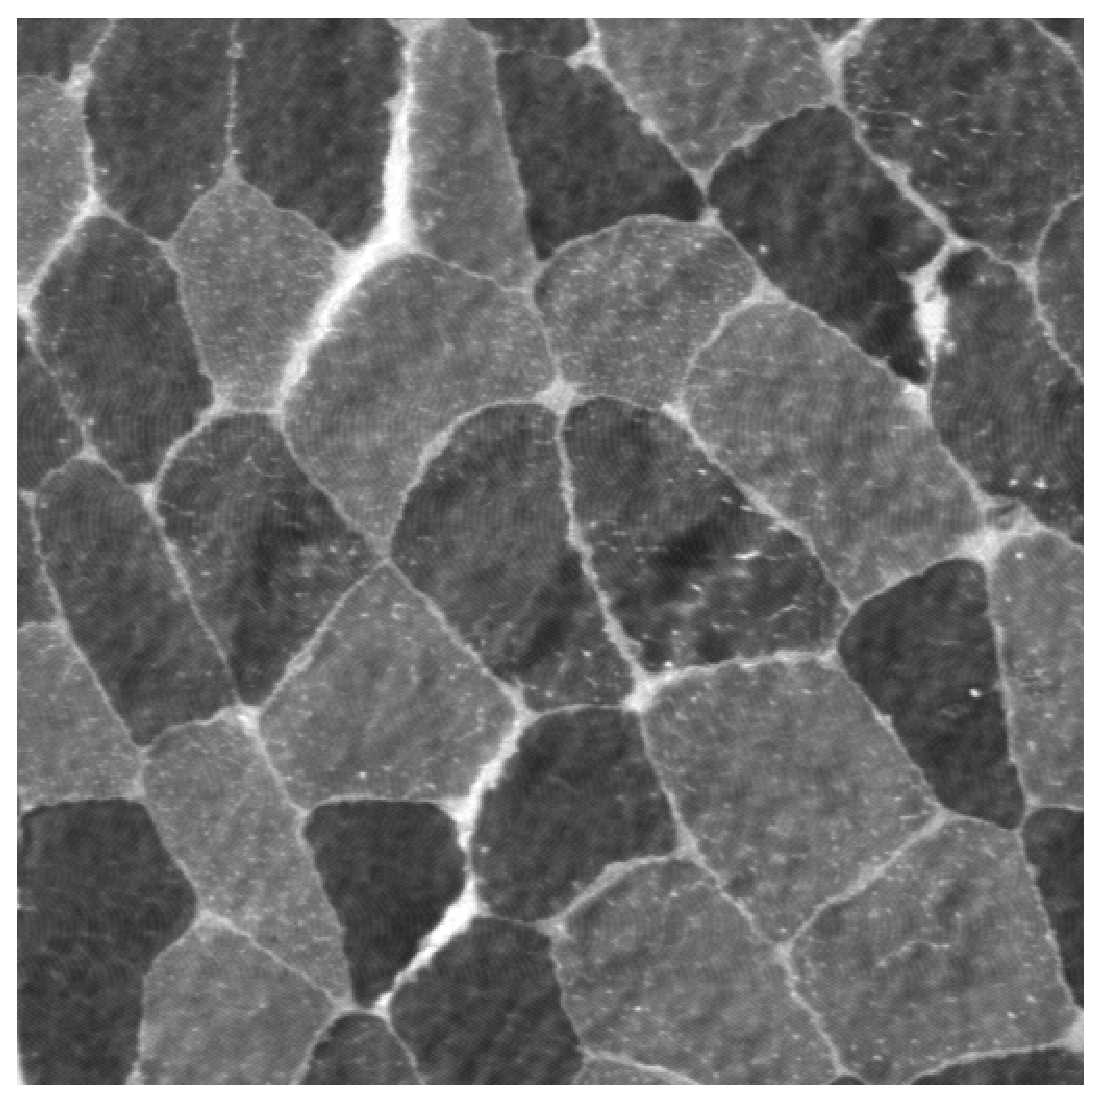
\includegraphics[width=2.5in]{./img/MUSCLEorig.eps}
  \caption{Ejemplo de una figura, pie de la fotografía, imagen en formato .eps}
  \label{fig:fig_sim}
\end{figure}




% Un ejemplo de tabla flotante. Para las tablas con estilo IEEE,  
% El comando \caption debe venir antes que comience la definición de la tabla
% El comando \label debe ir luego del comando \caption as siempre.
%
\begin{table}
% Ajusta el espaciado entre filas
  \renewcommand{\arraystretch}{1.3}
  \caption{Un ejemplo de tabla}
  \label{Etiqueta para el ejemplo de tabla}
  \centering
% definición de la tabla
  \begin{tabular}{|c||c|}
    \hline
      Fila 1, columna 1 & Fila 2, columna 2\\
    \hline
      Fila 2, columna 1 & Fila 2, columna 2\\
    \hline
  \end{tabular}
\end{table}


\section{Conclusión}
Gracias a la difusión del uso de ordenadores y programas de diseño gráfico, los textos simulados ganaron en popularidad. Mientras que antiguamente se repetían solamente algunas líneas del Lorem ipsum para crear un texto simulado, hoy en día el texto completo de Cicerón sirve como base para numerosos generadores de texto simulado o Lorem ipsum. Estos generadores pueden producir automáticamente fragmentos más largos del texto Lorem ipsum o de otros textos de relleno.

%Aquí va el apéndice
\appendices
\section{Título de la sección I dentro del apéndice}
Reconocimiento automático de un Lorem ipsum durante el trabajo de pre-prensa

Gracias a la difusión del uso de ordenadores y programas de diseño gráfico, los textos simulados ganaron en popularidad. Mientras que antiguamente se repetían solamente algunas líneas del Lorem ipsum para crear un texto simulado, hoy en día el texto completo de Cicerón sirve como base para numerosos generadores de texto simulado o Lorem ipsum. Estos generadores pueden producir automáticamente fragmentos más largos del texto Lorem ipsum o de otros textos de relleno.

\section{Título de la sección II dentro del apéndice}
Aquí va el segundo apéndice con un texto de relleno.


\section*{Agradecimientos}
Esta es una sección opcional, se colocan nombres de personas e instituciones que hicieron posible la investigación.

% Esta es una bibliografía de prueba, obtenida a partir de la primera plantilla

\begin{thebibliography}{1}

\bibitem{IEEEhowto:kopka}
H.~Kopka and P.~W. Daly, \emph{A Guide to {\LaTeX}}, 3rd~ed.\hskip 1em plus
  0.5em minus 0.4em\relax Harlow, England: Addison-Wesley, 1999.

\end{thebibliography}


%Sección de la biografía
\begin{biography}{Michael Shell}
Biography text here.
\end{biography}




\end{document}


